\section{Nguyên hàm}
\subsection{Đề 1}
\Opensolutionfile{ans}[ans/ans-2-B11-De1]
\caulc
%Câu 1
\begin{ex}%[Đề 12 - 2025 - Nguyen Son]%[2D4N1-4]
	Họ tất cả các nguyên hàm của hàm số $f(x)=\mathrm{e}^{5x}$ là
	\choice
	{$\mathrm{e}^{5x}\ln5$}
	{\True $\dfrac{1}{5} \mathrm{e}^{5x}+C$}
	{$5\mathrm{e}^{5x}+C$}
	{$\mathrm{e}^{5x}$}
	\loigiai {
		$\displaystyle\int f(x)\mathrm{\,d}x=\displaystyle\int \mathrm{e}^{5x}\mathrm{\,d}x=\dfrac{1}{5}\mathrm{e}^{5x}+C$.
	}
\end{ex}
%Câu 2
\begin{ex} %[Đề 12 - 2025 - Nguyen Son]%[2D4H1-4]
	Nguyên hàm $F(x)$ của hàm số $f(x)= \mathrm{e}^x - 3\mathrm{e}^{-x}$ thỏa mãn $F(0)=4$ là
	\choice
	{$F(x)=\mathrm{e}^x - 3\mathrm{e}^{-x}$}
	{$F(x)=\mathrm{e}^x + 3\mathrm{e}^{-2x}$}
	{\True $F(x)=\mathrm{e}^x + 3\mathrm{e}^{-x}$}
	{$F(x)=\mathrm{e}^x + 3\mathrm{e}^{-x} +4$}

\loigiai{
	$F(x)= \displaystyle \int f(x)\mathrm{\,d}x = \displaystyle \int \left(\mathrm{e}^x -3\mathrm{e}^{-x}\right) \mathrm{\,d}x = \mathrm{e}^x + 3\mathrm{e}^{-x} +C $ với $(C\in \mathbb{R})$.\\
	Ta có $F(0)=4$ suy ra $ \mathrm{e}^0 + 3\mathrm{e}^0 +C = 4 \Leftrightarrow C=0 $\\
	$\Rightarrow F(x) =\mathrm{e}^x + 3\mathrm{e}^{-x} $.
}
\end{ex}
%Câu 3
\begin{ex}%[Đề 12 - 2025 - Nguyen Son]%[2D4H1-2]
	Biết $F(x)$ là một nguyên hàm của $f(x)=\dfrac{1}{x-1}$ và $F(2)=1$. Tính $F(3)$.
	\choice
	{$F(3) =\ln 2 - 1$}
	{\True $F(3) =\ln 2 + 1$}
	{$F(3) =\dfrac{1}{2}$}
	{$F(3) =\dfrac{7}{4}$}
	\loigiai{
		Ta có $F(x) =\displaystyle\displaystyle\int f(x)\mathrm{d}x =\displaystyle\displaystyle\int\dfrac{1}{x - 1}\mathrm{d}x =\ln | x - 1 | + C$.\\
		Giả thiết $F(2) = 1\Rightarrow\ln 1 + C = 1\Rightarrow C = 1$.\\
		Suy ra $F(x) =\ln | x - 1 | + 1$. Vậy  $F ( 3 ) = \ln 2 + 1$.
		}
\end{ex}


%Câu 4
\begin{ex}%[Đề 12 - 2025 - Nguyen Son]%[2D4H1-4]
	Họ tất cả các nguyên hàm của hàm số $f(x)=2^{2x}\cdot 3^x\cdot 7^x$ là
	\choice
	{\True $\dfrac{84^x}{\ln 84}+C$}
	{$\dfrac{2^{2x}\cdot 3^x\cdot 7^x}{\ln2\cdot\ln3\cdot\ln7}+C$}
	{$84^x+C$}
	{$84^x\cdot\ln84+C$}
	\loigiai {
		$\displaystyle\int f(x)\mathrm{\,d}x=\displaystyle\int 2^{2x}\cdot 3^x\cdot 7^x\mathrm{\,d}x=\displaystyle\int 84^x\mathrm{\,d}x=\dfrac{84^x}{\ln 84}+C$.
	}
\end{ex}

%Câu 5
\begin{ex}%[Đề 12 - 2025 - Nguyen Son]%[2D4H1-2]
	Họ tất cả các nguyên hàm của hàm số $f(x)=\dfrac{x^2+3x+2}{x+3}$ trên khoảng $(-3;+\infty)$ là
	\choice
	{\True $\dfrac{x^2}{2}+2\ln(x+3)+C$}
	{$x+2\ln(x+3)+C$}
	{$\dfrac{x^2}{2}+\ln(x+3)+C$}
	{$\dfrac{x^2}{2}-2\ln(x+3)+C$}
	\loigiai{
		Ta có
		$$\displaystyle\int f(x)\mathrm{\,d}x=\displaystyle\int\dfrac{x^2+3x+2}{x+3}\mathrm{\,d}x=\displaystyle\int\left(x+\dfrac{2}{x+3}\right)\mathrm{\,d}x=\dfrac{x^2}{2}+2\ln|x+3|+C.$$
		Vì $x\in(-3;+\infty)$ nên $|x+3|=x+3$.\\
		Do đó $\displaystyle\int f(x)\mathrm{\,d}x=\dfrac{x^2}{2}+2\ln(x+3)+C$.}
\end{ex}
%Câu 6
\begin{ex}%[Đề 12 - 2025 - Nguyen Son]%[2D4H1-2]
	Họ nguyên hàm của hàm số $f(x) = \dfrac{1}{2x^2-3x+1}$ là
	\choice
	{$\displaystyle\int f(x) \mathrm{\,d}x =\dfrac{1}{2}\ln \left|\dfrac{x-1}{2x-1}\right|+C$}
	{$\displaystyle\int f(x) \mathrm{\,d}x =\dfrac{1}{3}\ln \left|\dfrac{x+2}{x-1}\right|+C$}
	{$\displaystyle\int f(x) \mathrm{\,d}x =\ln \left|\dfrac{x-1}{x-0,5}\right|+C$}
	{\True $\displaystyle\int f(x) \mathrm{\,d}x =\ln \left|\dfrac{x-1}{2x-1}\right|+C$}
	\loigiai{
		$\displaystyle\int \dfrac{1}{2x^2-3x+1}\mathrm{\,d}x=\displaystyle\int \dfrac{1}{(x-1)(2x-1)}\mathrm{\,d}x=\ln \left|\dfrac{x-1}{2x-1}\right|+C$.}
\end{ex}
%Câu 7
\begin{ex}%[Đề 12 - 2025 - Nguyen Son]%[2D4V1-3]
	Biết $\displaystyle  \int(2\sin x + \cos x)^2\mathrm{\, d}x=a \sin 2x - \cos 2x + bx +C$, với $a,b \in \mathbb{Q}$. Tính $a^2+b^2$.
	\choice
	{$\dfrac{17}{2}$}
	{$\dfrac{109}{4}$}
	{$\dfrac{17}{16}$}
	{\True $\dfrac{109}{16}$}
	\loigiai{
			\begin{eqnarray*}
				\displaystyle  \int(2\sin x + \cos x)^2\mathrm{\, d}x
				&=&\displaystyle  \int(4\sin^2x+4\sin x \cos x + \cos^2 x)\mathrm{\, d}x\\
				&=&\displaystyle  \int\left( 2\sin2x-\dfrac{3}{2}\cos 2x+\dfrac{5}{2}\right) \mathrm{\, d}x\\
				&=& -\dfrac{3}{4}\sin 2x - \cos 2x +\dfrac{5}{2}x+C.
			\end{eqnarray*}
			Suy ra $a=-\dfrac{3}{4}$ và $b=\dfrac{5}{2}$. Từ đó tính được $a^2+b^2=\dfrac{109}{16}$.}
	\end{ex}
%Câu 8
\begin{ex}%[Đề 12 - 2025 - Nguyen Son]%[2D4H1-3]
	Cho hàm số $f(x)$ thỏa mãn đồng thời các điều kiện $f'(x)=x+\sin x$ và $f(0)=1$. Tìm $f(x)$.
	\choice
	{$f(x)=\dfrac{x^2}{2}+\cos x$}
	{$f(x)=\dfrac{x^2}{2}-\cos x-2$}
	{\True $f(x)=\dfrac{x^2}{2}-\cos x+2$}
	{$f(x)=\dfrac{x^2}{2}+\cos x+\dfrac{1}{2}$}
	\loigiai{
		Ta có $f(x)=\displaystyle\int f'(x) \mathrm{\,d}x=\displaystyle\int (x+\sin x) \mathrm{\,d}x=\dfrac{x^2}{2}-\cos x+C$.\\
		Mà $f(0)=1\Rightarrow -1+C=1\Leftrightarrow C=2$.\\
		Vậy $f(x)=\dfrac{x^2}{2}-\cos x+2$.
	}
\end{ex}


%Câu 9
\begin{ex}%[Đề 12 - 2025 - Nguyen Son]%[2D4H1-3]
	Một nguyên hàm $F(x)$ của hàm số $f(x)=\sin x+\dfrac{1}{\cos^2 x}$ thỏa mãn $F\left(\dfrac{\pi}{4}\right)=\dfrac{\sqrt2}{2}$ là 
	\choice
	{ $-\cos x+\tan x+C$}	
	{$-\cos x+\tan x-\sqrt2 +1$}
	{$\cos x+\tan x+\sqrt2 -1$}
	{\True $-\cos x+\tan x+\sqrt2 -1$}
	\loigiai{
		Ta có $F(x)=\displaystyle\int\limits \left( \sin x+\dfrac{1}{\cos^2 x}  \right)\mathrm{\,d}x=-\cos x+\tan x+C$.\\
		Vì $F\left(\dfrac{\pi}{4}\right)=\dfrac{\sqrt2}{2}$ nên $C=\sqrt2-1$.\\
		Vậy  $F(x)=-\cos x+\tan x+\sqrt2 -1$.
	}
\end{ex}

%Câu 10
\begin{ex}%[Đề 12 - 2025 - Nguyen Son]%[2D4H1-2]
	Biết $F(x)$ là một nguyên hàm của hàm số $f(x)=\dfrac{1+2x^2}{x}$ thỏa mãn $F(-1)=3$. Khẳng định nào sau đây đúng?
	\choice
	{$F(x)=\ln|x|+x+2$}
	{$F(x)=\ln|x|+x^2-2$}
	{$F(x)=\ln|x|+2x^2+1$}
	{\True $F(x)=\ln|x|+x^2+2$}
	\loigiai
	{
		Ta có $F(x)=\displaystyle\int \dfrac{1+2x^2}{x}\mathrm{\,d}x=\displaystyle\int \left(\dfrac{1}{x}+2x\right)\mathrm{\,d}x=\ln|x|+x^2+C$.\\
		Mà $F(-1)=3\Leftrightarrow \ln|-1|+(-1)^2+C=3\Leftrightarrow C=2$.\\
		Vậy $F(x)=\ln|x|+x^2+2$.
	}
\end{ex}

%Câu 11
\begin{ex}%[Đề 12 - 2025 - Nguyen Son]%[2D4H1-1]
	Cho hàm số $ f(x) $ có đạo hàm $ f'(x) $ liên tục và có một nguyên hàm là hàm số $ F(x) $. Tìm nguyên hàm $ I=\displaystyle\int \left[2f(x)+f'(x)+1\right]\mathrm{d}x $.
	\choice
	{\True $ I=2F(x)+f(x)+x+C $}
	{$ I=2F(x)+xf(x)+C $}
	{$ I=2xF(x)+f(x)+x+1 $}
	{$ I=2xF(x)+f(x)+x+C $}
	\loigiai{
		Ta có $ I=\displaystyle\int \left[2f(x)+f'(x)+1\right]\mathrm{d}x=2F(x)+f(x)+x+C $.
	}
\end{ex}
%Câu 12
\begin{ex}%[Đề 12 - 2025 - Nguyen Son]%[2D4H1-3]
	Cho hàm số $ f(x)=\dfrac{1}{\sin^2 x} $. Nếu $ F(x) $ là một nguyên hàm của hàm số $ f(x) $ và đồ thị hàm số $ F(x) $ đi qua điểm $ M\left(\dfrac{\pi
	}{6}; 0\right) $ thì $ F(x) $ là
	\choice
	{$ -\dfrac{\sqrt{3}}{3}+\cot x $}
	{$ -\sqrt{3}+\cot x $}
	{\True $ \sqrt{3}-\cot x $}
	{$ \dfrac{\sqrt{3}}{3}-\cot x $}
	\loigiai{
		Ta có $ F(x)=-\cot x+C $.\\
		Vì đồ thị của hàm số $ F(x) $ đi qua điểm $ M\left(\dfrac{\pi
		}{6}; 0\right) $ nên $ 0=-\cot\dfrac{\pi}{6}+C\Leftrightarrow C=\sqrt{3} $.\\
		Vậy $ F(x)=\sqrt{3}-\cot x $.
	}
\end{ex}

\Closesolutionfile{ans}
\indapan{6}{ans/ans-2-B11-De1}

\cauds
\Opensolutionfile{ans}[ans/ans-2-B11-De1-DS]
%Câu 1
\begin{ex}%[Đề 12 - 2025 - Nguyen Son]%[2D4H1-2]
	Biết $F(x)=x^3-3x^2+2x$ là một nguyên hàm của hàm số $f(x)$ trên $\mathbb{R}$.
	\choiceTF
	{\True $F(1)=0$}
	{$\displaystyle\int F(x)\mathrm{d}x=3x^2-6x+2$}
	{\True $f(x)=3x^2-6x+2$}
	{Nếu $G(x)$ cũng là một nguyên hàm của hàm số $f(x)$ trên $\mathbb{R}$ thì $F(x)=G(x)$}
	\loigiai{
		\begin{itemchoice}
			\itemch Đúng. Ta có $F(1)=1^3-3\cdot 1^2+2\cdot 1=0$.
			\itemch Sai. \\
			Ta có $\displaystyle\int F(x)\mathrm{d}x=\displaystyle\int\left(x^3-3x^2+2x\right)\mathrm{d}x=\displaystyle\int x^3\mathrm{d}x+\displaystyle\int -3x^2\mathrm{d}x+\displaystyle\int 2x\mathrm{d}x=\dfrac{1}{4}x^4-x^3+x^2+C$.
			\itemch Đúng. Vì $F(x)$ là nguyên hàm của $f(x)$ trên $\mathbb{R}$ nên $f(x)=F'(x)=\left(x^3-3x^2+2x\right)'=3x^2-6x+2$.
			\itemch Sai. Nếu $G(x)$ cũng là một nguyên hàm của hàm số $f(x)$ trên $\mathbb{R}$ thì $G(x)=F(x)+C$.
		\end{itemchoice}
	}
\end{ex}
%Câu 2
\begin{ex}%[Đề 12 - 2025 - Nguyen Son]%[2D4V1-2]
	Cho hàm số $f(x)$ xác định trên $\mathbb{R}\setminus\left\lbrace 1;4 \right\rbrace$ có $f'(x)=\dfrac{2x-5}{x^2-5x+4}$ thỏa mãn $f(3)=1-\ln 2$. 
	\choiceTF
	{$f'(5)=-\dfrac{5}{4}$}
	{\True $f'(x)=\dfrac{1}{x-1}+\dfrac{1}{x-4}$}
	{\True $f(x)=\ln|x-1|+\ln|x-4|+1-2\ln2$}
	{Giá trị $f(2)$ bằng $1+\ln2 $}
	\loigiai{
		\begin{itemchoice}
			\itemch Sai. $f'(5)=\dfrac{2\cdot 5-5}{5^2-5\cdot 5+4}=\dfrac{5}{4}$.
			\itemch Đúng. Phân tích $f'(x)$ ta được $f'(x)=\dfrac{1}{x-1}+\dfrac{1}{x-4}$.
			\itemch Đúng. \\
			$f(x)=\displaystyle\int f'(x)\mathrm{\,d}x=\displaystyle\int\dfrac{2x-5}{x^2-5x+4}\mathrm{\,d}x\\
			=\displaystyle\int\left(\dfrac{1}{x-1}+\dfrac{1}{x-4}\right)\mathrm{\,d}x=\ln|x-1|+\ln|x-4|+C$.\\
			 Theo giả thiết $f(3)=1-\ln2 \Rightarrow \ln 2 +C=1-\ln2 \Leftrightarrow C=1-2\ln2$.
			 \itemch Sai. Ta có $f(x)=\ln|x-1|+\ln|x-4|+1-2\ln2$. Suy ra $f(2)=1-\ln2$.
		\end{itemchoice}
	}
\end{ex}
%Câu 3
\begin{ex}%[Đề 12 - 2025 - Nguyen Son]%[2D4H1-2]
	Cho $F(x)=mx^3+(3m+2)x^2-4x+3$ là một nguyên hàm của $f(x)=3x^2+10x-4$.
	\choiceTF
	{\True Hai hàm số $F(x)$ và $f(x)$ đều có nguyên hàm với mọi giá trị của $m$}
	{Một nguyên hàm của $f(x)$ là $x^3+10x^2-4$}
	{\True Để hàm số $F(x)$ là một nguyên hàm của hàm số $f(x)$ thì $m=1$}
	{Phương trình $ F(x)=-4 $ có ba nghiệm phân biệt}
	\loigiai{		
		\begin{itemchoice}
			
			\itemch Đúng. Hai hàm số $F(x)$ và $f(x)$ là hai hàm đa thức nên đều có nguyên hàm với mọi giá trị của $m$.
			\itemch Sai. Nguyên hàm của $f(x)$ là $x^3+5x^2-4x+C$.
			\itemch Đúng.\\
			Ta có $F'(x)=3m{x^2}+2\left(3m+2\right)x-4$.\newline
			Để $F(x)$ là một nguyên hàm của $f(x)$ thì $F'(x)=f(x)\\
			\Rightarrow
			\heva{&3m=3\\&2\left(3m+2\right)=10\\&-4=-4}  \Leftrightarrow m=1.$
			\itemch Sai. Phương trình $ F(x)=-4 \Leftrightarrow x^3+5x^2=0 \Leftrightarrow x= 0$ hoặc $x=-5$. Do đó phương trình $ F(x)=-4 $ chỉ có hai nghiệm.
		\end{itemchoice}
	}
\end{ex}
%Câu 4
\begin{ex}%[Đề 12 - 2025 - Nguyen Son]%[2D4V1-6]
	\immini{
		Một vật chuyển động trong 4 giờ với vận tốc $v$ (km/h) phụ thuộc thời gian $t$ (h) có đồ thị của vận tốc như hình bên. Trong khoảng thời gian 3 giờ kể từ khi bắt đầu chuyển động, đồ thị đó là một phần của parabol có đỉnh $I\left(2;9\right)$ với trục đối xứng song song với trục tung, khoảng thời gian còn lại đồ thị là một đoạn thẳng song song với trục hoành.
	}{
		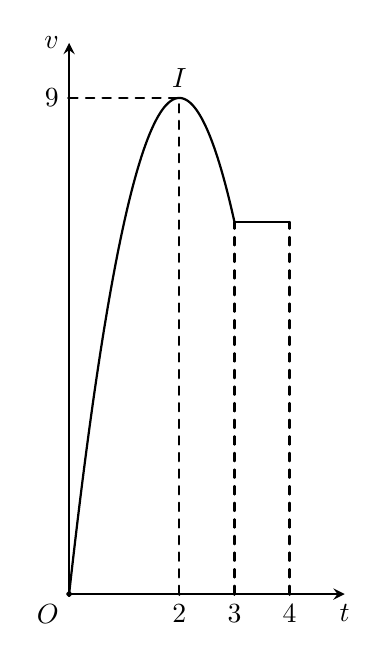
\begin{tikzpicture}[line join=round, line cap=round,>=stealth,thick,scale=0.7]
			
			\draw[->] (0,0)--(5,0) node[below] {$t$};
			\draw[->] (0,0)--(0,10) node[left] {$v$};
			\draw (0,0) node [below left] {$O$} circle(1pt);
			\draw[dashed] (2,0) -- (2,9) -- (0,9) (3,0)--(3,6.75) (4,0)--(4,6.75);
			\draw[samples=200,domain=0:3,smooth,variable=\x] plot (\x,{(-2.25)*(\x)^2 +9*(\x)});
			\draw[thick] (3,6.75)--(4,6.75);
			\fill 
			(0,9) node[left]{$9$} circle(1pt)
			(2,0) node[below]{$2$} circle(1pt)
			(3,0) node[below]{$3$} circle(1pt) 
			(4,0)node[below]{$4$} circle (1pt)
			(2,9)node[above]{$I$};
	\end{tikzpicture}}
	\choiceTF
	{\True Vận tốc lớn nhất của chuyển động là $9$ (km/h)}
	{\True $v(t)=-\dfrac{9}{4}t^2+9t$, với $0\leq t\leq 3$}
	{$v(t)=\dfrac{27}{4}t$, với $3\leq t\leq 4$}
	{\True Quãng đường vật di chuyển được trong 4 giờ là $27$ km}
	\loigiai{		
		\begin{itemchoice}
			\itemch Đúng. Dựa vào đồ thị hàm số ta có $\max\limits_{\left[0;4\right]}v=9$ khi $t=2$ h.
			\itemch Đúng. Với $0\leq t\leq 3$ ta có đồ thị vận tốc là một parabol. Vì parabol có đỉnh $I\left(2;9\right)$ nên parabol có phương trình dạng $y=a\left(t-2\right)^2+9$.\\
			Ta lại có parabol luôn đi qua gốc tọa độ nên $0=a(0-2)^2+9\Leftrightarrow a=-\dfrac{9}{4}$.\\
			Khi đó $y=-\dfrac{9}{a}\left(t-2\right)^2+9\Leftrightarrow y=-\dfrac{9}{4}t^2+9t$.
			\itemch Sai. Với $3\leq t\leq 4$ ta có đồ thị vận tốc là một đường thẳng song song với trục hoành nến $v=c$ với $c=v(3)=-\dfrac{9}{4}\cdot 3^2+9\cdot 3=\dfrac{27}{4}$.\\
			Vậy $y=\dfrac{27}{4}$ với $3\leq t\leq 4$.
			\itemch Đúng. Trong 4 giờ đầu vật chia thành 2 giai đoạn chuyển động.\\
			Giai đoạn 1, trong 3 giờ đầu ta có $s(t)=\displaystyle\int \left(-\dfrac{9}{4}t^2+9t\right)\mathrm{d}t=-\dfrac{3}{4}t^3+\dfrac{9}{2}t^2+c$.\\
			Vì $s(0)=0$ nên $c=0$. Suy ra, $s_{1}=s(3)=\dfrac{81}{4}$ km.\\
			Giai đoạn 2, từ giờ thứ 3 đến giờ thứ 4, ta có $s(t)=\displaystyle\int \dfrac{27}{4}\mathrm{d}t=\dfrac{27}{4}t+c'$. Vì $s(3)=\dfrac{81}{4}$ nên $c'=0$.\\ Suy ra, $s_2=s(4)-s(3)=\dfrac{27}{4}$.\\
			Vậy $s=s_1+s_2=27$ km.
		\end{itemchoice}
	}
\end{ex}
\Closesolutionfile{ans}
\indapan{3}{ans/ans-2-B11-De1-DS}

\Opensolutionfile{ans}[ans/ans-2-B11-De1-KQ]
\caukq
%Câu 1
\begin{ex}%[Đề 12 - 2025 - Nguyen Son]%[2D4H1-3]
	Cho hàm số $f(x)$ thỏa mãn $f'(x)=27+\cos x$ và $f(0)=25$. Tính $f(1)$. (Kết quả làm tròn đến hàng phần mười).
	\shortans{$52{,}8$}
	\loigiai{$f'(x)=27+\cos x\Rightarrow \displaystyle\int f'(x)\mathrm{\,d}x =\displaystyle\int (27+\cos x)\mathrm{\,d}x \Rightarrow f(x)=27x+\sin x+C$.\\
		Mà $f(0)=25\Rightarrow 27\cdot 0+\sin 0+C=25\Leftrightarrow C=25\Rightarrow f(x)=27x+\sin x+25.\\
		\Rightarrow f(1)=27\cdot 1+\sin 1+25\approx 52{,}8$.
	}
\end{ex}
%Câu 2
\begin{ex}%[Đề 12 - 2025 - Nguyen Son]%[2D4H1-2]
	Cho biết $\displaystyle\int\dfrac{4x+1}{2x+3}\mathrm{\,d}x=ax-\dfrac{b}{2}\ln(2x+3)+C$ với $x\in\left(-\dfrac{3}{2};+\infty\right)$ ($a$, $b$ là các số nguyên dương). Tính $2a-b$.
	\shortans{$-1$}
	\loigiai{
		Ta có: $\displaystyle\int\dfrac{4x+1}{2x+3}\mathrm{\,d}x=\displaystyle\int\left(2-\dfrac{5}{2x+3}\right)\mathrm{\,d}x=2x-\dfrac{5}{2}\ln|2x+3|+C$.\\
		Vì $x\in\left(-\dfrac{3}{2};+\infty\right)$ nên $|2x+3|=2x+3$.\\
		Do đó $\displaystyle\int\dfrac{4x+1}{2x+3}\mathrm{\,d}x=2x-\dfrac{5}{2}\ln(2x+3)+C$. Vậy $a=2$, $b=5$, suy ra $2a-b=-1$.}
\end{ex}
%Câu 3
\begin{ex}%[Đề 12 - 2025 - Nguyen Son]%[2D4H1-1]
	Gọi $F(x)=(ax^2+bx+c)\mathrm{e}^x$ là một nguyên hàm của hàm số $f(x)=(x-1)^2\mathrm{e}^x$. Tính $S=a+2b+c$.
	\shortans{$-2$}
	\loigiai{
		Ta có $F'(x)=(ax^2+bx+c)\mathrm{e}^x+(2ax+b)\mathrm{e}^x=[ax^2+(2a+b)x+b+c]\mathrm{e}^x$.\\
		Và $f(x)=(x^2-2x+1)\mathrm{e}^x$.\\
		Đồng nhất hệ số với $f(x)$ ta có
		$$\heva{& a=1 \\ & 2a+b=-2\\& b+c=1}\Leftrightarrow \heva{& a=1 \\ & b=-4\\ & c=5.}$$
		Vậy $a+2b+c=-2$.
	}
\end{ex}
%Câu 4
\begin{ex}%[Đề 12 - 2025 - Nguyen Son]%[2D4V1-6]
	Một vật chuyển động có gia tốc là $a\left(t\right)=3 t^2+t$ (m/s$^2$). Biết rằng vận tốc ban đầu của vật là $2$ m/s. Vận tốc của vật đó sau $4$ giây là bao nhiêu (m/s)?
	\shortans{$74$}
	\loigiai{
		Vận tốc của vật là $v(t)=\displaystyle \int \left(3 t^2+t\right)  \mathrm{\,d}t =t^3+\dfrac{1}{2}t^2+C$.\\
		Vì vận tốc tốc ban đầu của vật là $2$ m/s nên $v(0)=2 \Leftrightarrow 0^3+\dfrac{1}{2}\cdot 0^2+C=2  \Leftrightarrow C=2$.\\
		Suy ra $v(t)=t^3+\dfrac{1}{2}t^2+2$.\\
		Vận tốc của vật đó sau $4$ giây là $v(4)=4^3+\dfrac{1}{2}\cdot 4^2+2=74$ (m/s).
	}
\end{ex}
%Câu 5
\begin{ex}%[Đề 12 - 2025 - Nguyen Son]%[2D4V1-1]
	Cho hàm số $f(x)$ có đạo hàm liên tục trên $[1;4]$ thỏa mãn $f(1)=2$ và $f(x)=x^3+1-xf'(x)$. Tính $f(4)$ (Kết quả làm tròn đến hàng phần mười).
	\shortans{$17{,}2$}
	\loigiai{
		Xét	
		\begin{eqnarray*}
			f(x)=x^3+1-xf'(x) 
			&\Leftrightarrow&f(x)+xf'(x)=x^3+1\\
			&\Leftrightarrow& [xf(x)]'=x^3+1 \Leftrightarrow xf(x)=\dfrac{x^4}{4}+x+C \quad(1)
		\end{eqnarray*}
		Thay $x=1$ vào (1), ta được $1\cdot f(1)=\dfrac{1}{4}+1+C \Rightarrow C=\dfrac{3}{4}$. \\
		Vậy $xf(x)=\dfrac{x^4}{4}+x+\dfrac{3}{4} \Rightarrow f(4)=\dfrac{275}{16}\approx 17{,}2$.
	}
\end{ex}

%Câu 6
\begin{ex}%[Đề 12 - 2025 - Nguyen Son]%[2D4V1-1]
	Cho hàm số $y=f(x)$ có đạo hàm liên tục trên $[1;2]$ thỏa mãn $f(1)=4$ và $f(x)=xf'(x)-2x^3-3x^2$. Tính $f(2)$.
	\shortans{$20$}
	\loigiai{
		Với $x\in [1;2]$ ta có 
		\begin{eqnarray*}
			f(x)=xf'(x)-2x^3-3x^2 &\Leftrightarrow& \dfrac{xf'(x)-f(x)}{x^2}=2x+3\\
			&\Leftrightarrow& \left(\dfrac{f(x)}{x}\right)'=2x+3\\
			&\Leftrightarrow& \dfrac{f(x)}{x}=x^2+3x+C.
		\end{eqnarray*}
		Do $f(1)=4$ nên $C=0 \Rightarrow f(x)=x^3+3x^2$. \\
		Vậy $f(2)=2^3+3\cdot 2^2=20$.
	}
\end{ex}
\Closesolutionfile{ans}
\indapan{6}{ans/ans-2-B11-De1-KQ}